\documentclass[journal]{IEEEtran}
\usepackage{blindtext}
\usepackage{graphicx}
\usepackage[justification=centering]{caption}


\ifCLASSINFOpdf
  % \usepackage[pdftex]{graphicx}
  % declare the path(s) where your graphic files are
  % \graphicspath{{../pdf/}{../jpeg/}}
  % and their extensions so you won't have to specify these with
  % every instance of \includegraphics
  % \DeclareGraphicsExtensions{.pdf,.jpeg,.png}
\else
  % or other class option (dvipsone, dvipdf, if not using dvips). graphicx
  % will default to the driver specified in the system graphics.cfg if no
  % driver is specified.
  % \usepackage[dvips]{graphicx}
  % declare the path(s) where your graphic files are
  % \graphicspath{{../eps/}}
  % and their extensions so you won't have to specify these with
  % every instance of \includegraphics
  % \DeclareGraphicsExtensions{.eps}
\fi
% graphicx was written by David Carlisle and Sebastian Rahtz. It is
% required if you want graphics, photos, etc. graphicx.sty is already
% installed on most LaTeX systems. The latest version and documentation can
% be obtained at: 
% http://www.ctan.org/tex-archive/macros/latex/required/graphics/
% Another good source of documentation is "Using Imported Graphics in
% LaTeX2e" by Keith Reckdahl which can be found as epslatex.ps or
% epslatex.pdf at: http://www.ctan.org/tex-archive/info/
%

\begin{document}
\title{IS593 Term Project \emph{"Find Universal Cross Site Scripting Vulnerabilities in Brave Browser"}}

\author{Antoine RONDELET (20176461)}
\maketitle
\IEEEpeerreviewmaketitle

\section{Introduction}
[TODO]\\

In the previous work, we can speak about the CVEs and the paper \cite{uxssJSLeaks}.

Write the introduction at the end
Finish the introduction by a list of keywords.

It might be good to begin the paper with a bit of context about UXSS research. See whether we manage to find some papers about it -> if yes: speak about previous work, if no: speak about the fact that we couldn't find anything and that we were surprised to see that no previous work were carried out to try to study the security mechanisms of browsers and that current UXSS investigations are carried out by either companies themselves or by isolated persons reporting bugs to companies. This paper is an attempt to study browser's vulnerability, especially Universal XSS vulnerabilities.

Maybe do a small introduction about us (the team) and say that we are students in the computer science and information security departments at KAIST. Passionate by security and cryptography we decided to study UXSS. We have a very small background in Web programming and didn't know that much about the way browsers worked before this study, however, the potential theat behind UXSS attacks attracted our attention, and further to some research, it turned out that UXSS investigations were carried out by either companies themselves or by isolated persons reporting bugs to companies. Thus, our paper is an first attempt to study browser's vulnerability, especially Universal XSS vulnerabilities, and gather what we found. 

\section{Web Browsers}

\subsection{Role}
Before presenting our work, we want to define what exactly a browser is and what is its intrinsic role. \\
According to Wikipedia, a web browser (commonly referred to as a browser) is a software application for retrieving, presenting and traversing information resources on the World Wide Web.\footnote{https://en.wikipedia.org/wiki/Web\_browser} 
While the primary role of these pieces of software is to provide an easy way for users to access web resources, most of today's web browsers implement a myriad of features such as the support for secure communications, the possibility to execute Javascript code or even the ability to be extended with plugins, to only name a few.

\begin{figure}[h]
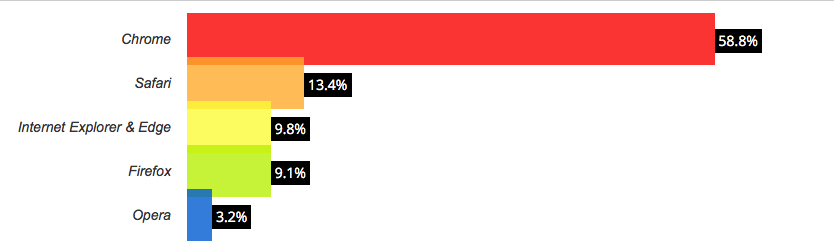
\includegraphics[width=0.4\textwidth]{images/WebBrowserMarketShare.png}
\caption{Web Browser Market Share in October 2017 \\ (from www.w3counter.com)}
\label{fig:marketShare}
\end{figure}

Around two decades after Netscape's Navigator and Window's Internet Explorer \emph{Browser wars}, the competition is still prevailing on the web browser market. The democratization of the use of the Web and, more recently, the introduction of HTML5, CSS3, and extensive client-side scripting to the World Wide Web, as well as more widespread use of smartphones and other mobile devices for browsing the web, lead to the apparition of dozens of browsers. From Mozilla's Firefox\footnote{https://www.mozilla.org/en-US/firefox/}, Google's Chrome\footnote{https://www.google.com/chrome/index.html}, Apple's Safari\footnote{https://www.apple.com/safari/} to Opera\footnote{http://www.opera.com/fr} for the most famous, the number of new browsers never ceases to increase. Today, as we are moving to the 4th industrial revolution - where data is moving astoundingly fast, and collected massively to be fed into \emph{Intelligent Agents} - some newcomers such as Brave\footnote{https://brave.com} or even Whale\footnote{http://whale.naver.com/en/} are trying to enter this disputed market and get their slice of the cake.
Although, figures \ref{fig:marketShare} and \ref{fig:monthlyUsage} agree on the fact that Google Chrome is the most widespread browser, other companies are working hard and hiring massively to try to dethrone Google's super star.

\begin{figure}[h]
\centering
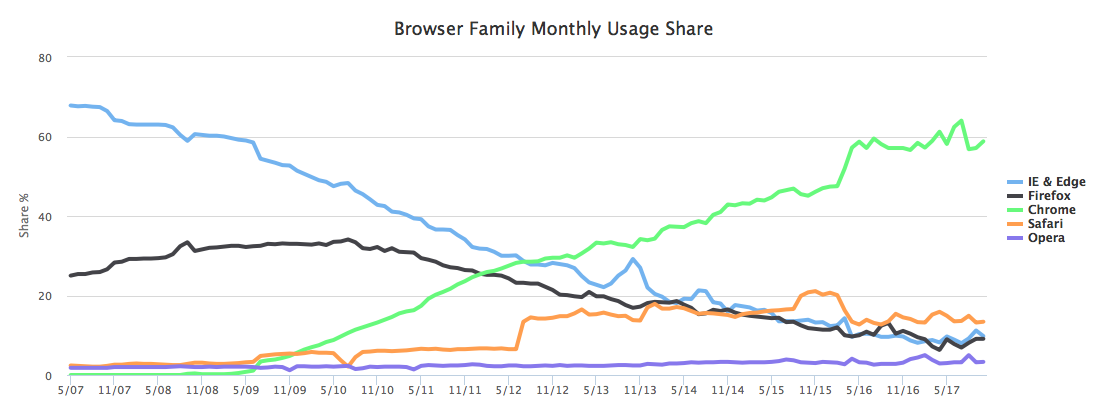
\includegraphics[width=0.4\textwidth]{images/BrowserFamilyMonthlyUsageShare.png}
\caption{Web Browser Monthly Usage Share \\ (from www.w3counter.com)}
\label{fig:monthlyUsage}
\end{figure}


As opposed to Netscape's Navigator, today, most web browsers are free to use. Developing web browsers is not about making money anymore, but more about sculpting people's computing habits in a way that would benefit the companies behind them.
As the market is quite competitive, developing a web browser can be seen as taking part into a race to developing the most features. This willingness to be different and attract people's attention often lead web browsers developers to implement features in a hurry. Such frequent releases sometimes unveil exploitable vulnerabilities and make browser's architecture more and more complex.

\medskip

A taste of a web browser's design is provided in the next part of this paper.

\subsection{Architecture}

Despite the large variety of browsers available to surf the web, most of them tend to follow a general structure. This architecture, as shown in \cite{architectureWebBrowsers} \cite{howBrowsersWork} can be decomposed into eight components, each of which has its very own functionality.

\subsubsection{User Interface}
The component in charge of the UI contains every piece of the browser that is not actually part of the webpage itself. Such piece can either be toolbars or Back and forward buttons for instance.

\subsubsection{Browser Engine}
The browser engine forms the interface that allows the User Interface to interact and manipulate elements of the rendering engine. It basically marshals actions between the UI and the rendering engine.

\subsubsection{Rendering Engine}
The rendering engine is responsible for producing a graphical representation of the document fetched from a specific URL. It parses and render documents written in HTML and applies styles specified by CSS.

\subsubsection{Data Persistence}
The data persistence subsystem is responsible for insuring the persistence of data when the browser needs it. For instance, a browser needs to save data locally to keep track of the user's bookmarks and cookies.

\subsubsection{Networking}
Since a browser fetches document from the Web, a browser needs to be able to have an access to the network. This access is provided by the networking module. It implements file transfer protocols such as HTTP and FTP. Moreover, this subsystem translates between different character sets, and resolves MIME media types for files\footnote{https://en.wikipedia.org/wiki/Media\_type}. In some cases, the networking module might also implement a cache of recently retrieved resources to ensure good performances when a user asks multiple times the same resource.

\subsubsection{Javascript Interpreter}
This module parses and executes Javascript\footnote{Programming language developed by Netscape in 1995 to make webpages interactive. More details can be found at https://en.wikipedia.org/wiki/JavaScript} code.

\subsubsection{XML parser}
The XML parser module is in charge of parsing XML documents into a Document Object Model (DOM) tree\footnote{https://en.wikipedia.org/wiki/Document\_Object\_Model}

\subsubsection{Display Backend}
The display backend subsystem provides primitives for drawing and windows. It also interfaces with the Operating System of the host machine.

\begin{figure}[h]
\centering
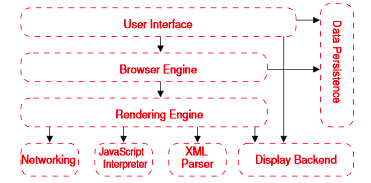
\includegraphics[width=0.4\textwidth]{images/BrowserStructure.png}
\caption{General Web Browser Structure}
\label{fig:browserStructure}
\end{figure}

While figure \ref{fig:browserStructure} shows the general web browser structure explained above, it is without saying that each browser has its particularities and its very own version of the aforementioned architecture.

\medskip

At this point, the reader should be able to have a taste of the complexity of web browsers. Such a compound of subsystems might be likely to expose several vulnerabilities either in the subsystems' implementation or in their interactions.

\subsection{Security mechanisms}
While, the Internet today is a widespread information infrastructure, the Web is not only used to access and share resources, but is also hosting commercial activities. According to http://www.internetworldstats.com/stats.htm, 51.7\% of the world population\footnote{This represent 3,885,567,619 people} is now using the Internet on a day to day basis. Albeit, a vast majority of Internet users are undoubtedly honest users, a few of them are malicious and carry out attacks on the network or publish malicious web pages on the web waiting for users to fetch them. From this point, a malicious page displayed in victims' browser could run malicious Javascript code trying to retrieve user's sensitive data. \\
In fact, in general, many pages tend to be displayed in a user's browser at the same time (into tabs or iframes\footnote{https://developer.mozilla.org/en-US/docs/Web/HTML/Element/iframe}). Thus, they all live in the browser in the same time. So how about using the browser as a bridge for a malicious page to access sensitive data stored in other pages ? \\

Since browsers are the door that enable us to access web pages from a lot of sources every day, such a vulnerability would be a major threat for Internet users. Being able to keep browsers safe from such menaces is paramount to keep the web safe. In order to do so, web browsers developers developed very sophisticated security mechanisms to isolate web pages from one another.

Moreover, modern web browsers need to support the latest and constantly evolving web standards capable of loading resources, while making sure that their level of security remains optimal. As a matter of fact, as explained in \cite{browserSecurity}, web browsers are committed to implement most of the security specifications defined by the World Wide Web Consortium (W3C), such as: (see \cite{SOP} \cite{CORS} \cite{CSP} \cite{SRI} \cite{MixedContent})

\medskip

\subsubsection{Same Origin Policy (SOP)}

The foundation of browsers security mechanisms is the notion of Same Origin Policy (referred to as SOP). Before looking at this important concept, we should first define what an origin is.

\medskip

In order to access a specific resource, a user has to specify its Uniform Resource Locator (URL)\footnote{Reference to a web resource that specifies its location on a computer network and a mechanism for retrieving it.}. This web address is a compound of different elements, as shown on figure \ref{fig:URL}. The protocol indicates which protocol the browser must use to retrieve the resource. The domain name is an alias for the IP address pointing to the Web server that should be requested. The port is a logical construct that identifies a specific process or a type of network service, on the web server, that is responsible for serving the web resource. Moreover, the path, parameters and fragment are the path to the resource on the Web server, extra parameters provided to the Web server and an anchor to a specific part of the resource itself, respectively.

\begin{figure}[h]
\centering
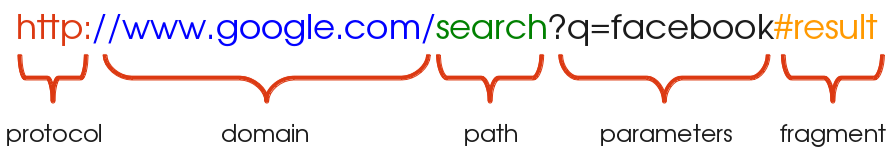
\includegraphics[width=0.4\textwidth]{images/URL.png}
\caption{URL anatomy}
\label{fig:URL}
\end{figure}

\medskip

With this in mind, defining what an origin is becomes trivial. Looking at the official definition of the W3C\footnote{https://www.w3.org/Security/wiki/Same\_Origin\_Policy}, an origin is defined by the scheme, host, and port of a URL.

\medskip

Know that we know what an origin is, the Same Origin Policy is a policy that ensures that documents retrieved from distinct origins are isolated from each other. Thus, even if users happened to visit malicious web sites, these fraudulent sites would not be able to interfere with the user's session with honest web sites.

\begin{figure}[h]
\centering
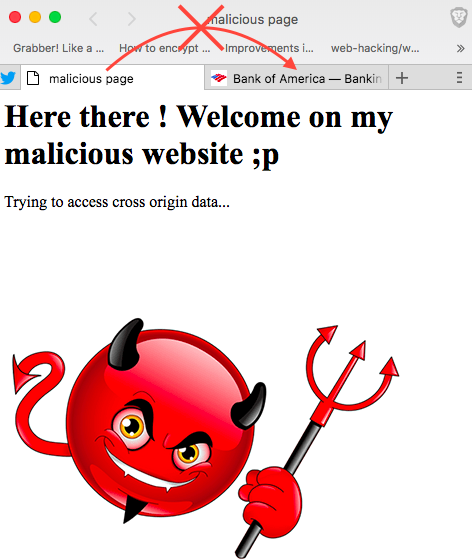
\includegraphics[width=0.4\textwidth]{images/SOPTabs.png}
\caption{Same Origin Policy preventing a malicious "tabs" to access user's sensitive data}
\label{fig:SOPTabs}
\end{figure}

\subsubsection{Cross-Origin Resource Sharing (CORS)}

In order to relax the SOP, the W3C specified the Cross-Origin Resource Sharing (CORS) which consists in specifying a white-list of trusted domains allowed to request restricted resources, by extending HTTP with a new origin request header. The CORS mechanism supports secure cross-domain requests and data transfers between browsers and web servers. \\

Even though, the policy is defined by web server administrators, this security mechanism is used in modern browsers especially on APIs such as \emph{XMLHttpRequest} or \emph{Fetch} to help mitigate the risks of cross-origin HTTP requests and prevent a malicious user to access a resource he should not be able to access.

\subsubsection{Content Security Policy (CSP)}

The Content Security Policy allows web site administrators to define a white-list in a HTTP header to specify trusted sources for delivering content. That way web authors can control resources the user agent is allowed to load for a given page.

\subsubsection{Mixed Content Blocking}

The mechanism of Mixed Content Blocking blocks insecure content on web pages that are considered secure. A "mixed" content can happen in the case where a user fetches a secure page over HTTPS, containing a HTTP content. Since data transiting over HTTP is not secure and can be eavesdropped, the Mixed Content Blocking mechanism will block this part of the web page. That way the page displayed to the user would be "completely safe from risks"\footnote{This section is placed into quotes because in web security, very few things (not to say nothing) are said to be unconditionally safe.}.

\subsubsection{Subresource Integrity (SRI)}

Subresource Integrity defines a mechanism by which user agents may verify that a fetched resource has been delivered without being altered. This process allow a User Agent to be sure that the requested resource is the one it received. SRI works by using hash functions. Website developers can associated a hash value to a specific resource. That way web browsers can compute the hash value of the received resource and compare them with the initial value provided by the website. The resource is then displayed only if the hash values are equal, i.e: the resource is valid. 

\medskip
\medskip

Despite the implementation and support of the security specifications of the W3C, some lower level attacks could be carried out to escape the security mechanisms of today's web browsers. By compromising a browser process and execute arbitrary code, and attacker could either be able to access the host system or bypass the SOP. The next subsections present the concepts of Sandboxes and Process and Origin Isolation, that are currently ensuring that low level attacks would not have dramatic impacts for end-users, and that SOP would not be "bypassable" at lower levels.

\subsection{Sandboxes}

Sandboxes is a mechanism which consists in limiting vulnerabilities by isolating components of an application from each other and from the rest of the system. In a sandbox, components run with the minimum access privileges to system resources they need to perform their functions.
By isolating complex components into sandboxes, web browser developers can diminish the impact vulnerabilities can have for the end-user. By limiting the damages an attacker can cause. \\

Some additional pieces of information about Google Chrome's sandboxes are provided in \cite{browserSecurityWhitePaper}, and an extract is illustrated in figure \ref{fig:ChromeSandboxes}.

\begin{figure}[h]
\centering
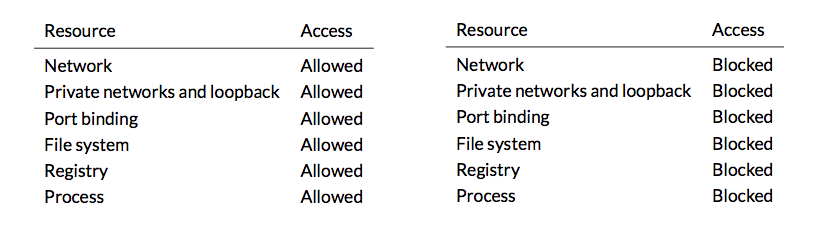
\includegraphics[width=0.4\textwidth]{images/SandboxesChrome.png}
\caption{Left: Google Chrome Main Process Sandbox, Right: Google Chrome Render Sandbox}
\label{fig:ChromeSandboxes}
\end{figure}

\subsection{Process and Origin Isolation}

We studied the mechanism of Same Origin Policy earlier in this paper. This concept restricts access to data across webpages if they have different origins. While the SOP is generally implemented at a high level, an attacker able to achieve process-level attacks might be able to bypass the Same Origin Policy, and thus accessing resources of a different origin hosted in the same process. To void such scenarios, decided to host each origin in a different process. That way by preventing direct access between these processes, and applying the same-origin policy in the APIs used by these processes for inter-origin communications, the same-origin policy can be enforced at all levels in browsers. The idea here is to ensure a strong site isolation and establish strong security boundaries between web sites \cite{isolationChrome}.

\begin{figure}[h]
\centering
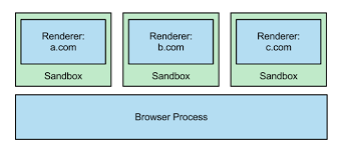
\includegraphics[width=0.4\textwidth]{images/IsolationChrome.png}
\caption{Site isolation in Chrome}
\label{fig:ChromeIsolation}
\end{figure}

\section{Universal XSS}

Despite all the security mechanisms used in today's browsers, some people still manage to find vulnerabilities that allow them to bypass the same-origin policy generically. Such vulnerabilities can lead to what is called Universal Cross-site Scripting (UXSS).
Before studying the Universal Cross Site Scripting attacks that have been carried out against modern web browsers, the next section defines what Cross Site Scripting (XSS) attacks are.

\subsection{\emph{"Classic"} XSS attack}

According to \cite{owaspXSS}, Cross-Site Scripting (XSS) attacks are a type of injection, in which malicious scripts are injected into benign and trusted web sites.
Since the end user’s browser has no way to know whether the script should be trusted or not, it will execute the script. As a matter of fact, injected code are executed at the attacker’s tar get origin. Thus, the malicious script can access any cookies, session tokens, or other sensitive information retained by the browser and associated with this origin. These scripts can even rewrite the content of the HTML page.

\bigskip

\fbox{\begin{minipage}{22em}
XSS attacks are injection attacks which exploit vulnerabilities in \textbf{web applications}.
\end{minipage}}

\bigskip

In order to carry out a cross-site scripting attack, a malicious user exploit a vulnerability found in the victim web application. Such vulnerability can be a lack of user input sanitizing which allow the user to send an inline script that is going to be executed or a regular expression that would enable a malicious website to send malicious \emph{postMessages}  \cite{postMessagesXSS} to a victim website embedded in an \emph{iframe}, for instance. 

\medskip

Since XSS attacks are one of the most popular attacks against web applications, developers are highly encouraged to implement good practices in order to prevent any damage engendered by cross-site scripting attacks. Nevertheless, as SOP is implemented by web browsers, a malicious user able to find a vulnerability in a web browser could bypass every defense of a web application, and thus inject malicious payload to any web page origin.

\subsection{UXSS: A major threat}

Universal XSS (UXSS) is a particular type of Cross-Site Scripting that has the ability to be triggered by exploiting flaws inside browsers, instead of leveraging the vulnerabilities against insecure web sites.

\bigskip

\fbox{\begin{minipage}{22em}
UXSS attacks exploit vulnerabilities in \textbf{web browsers}.
\end{minipage}}

\bigskip

In UXSS attacks, client-side vulnerabilities are exploited in a web browser or browser extensions to generate an XSS condition, which allows the malicious code to be executed, bypassing or disabling the security protection mechanisms in the web browser.

\medskip

The consequences of such an attack are pretty critical. In the case of a successful UXSS, the attacker doesn’t just get access to a compromised session on a vulnerable web page, but may get access to any session belonging to web pages currently opened (or cached) by the browser at the time the attack is triggered. UXSS does not need a vulnerable web page in order to trigger, and can penetrate web sessions belonging to secure, well written web pages. Thus, UXSS can create a vulnerability where there isn’t one !

\medskip

While bypassing all the security mechanisms described above in this paper might appear impossible, 
the attentive reader may remember that web browsers developers are in a popularity contest, and in order to be on top, need to implement numerous features over short periods of time. Even though security features are highly regarded, usability and integration features are usually easier to test and implement, and thus often done in priority. \\
Furthermore, UXSS attacks can also be carried out using vulnerabilities in plugins. This makes ensuring security of web browsers, an even more difficult task. Since a countless number of extensions are available to users they all constitute a potential security hole exploitable by attackers.


\section{Brave}

Now that we have defined what UXSS was and studied the consequences of such attacks, we now need to define the environment we used to carry out our project. \\
In order to conduct our study, we decided to choose the browser Brave\footnote{https://brave.com} which was first announced in January 2016. This free and open-source web browser is based on the Chromium\footnote{https://www.chromium.org} web browser. Brave is said to block website trackers, remove intrusive Internet advertisements, and also claims to improve online privacy by sharing less data with advertising customers. One specificity of Brave, is that the beta version is testing a new system to reward publishers, called Brave Payments. According to \cite{braveWikipedia}, this system allows users to optionally set a budget that they are willing to donate to the websites they visit. Brave then calculates the percentage assigned to each website through an algorithm and the publisher receives a transfer in bitcoins\footnote{https://bitcoin.org/en/}.

\medskip

Our willingness to carry out our project on Brave was due to the fact that this browser is pretty new (only one year) and still in Beta version. Moreover, the new features included into this browser and the small amount of reported vulnerabilities (see: figure \ref{fig:BraveReportedVulnerabilities}) opened the door for more vulnerabilities and made it a good candidate for our project.

\begin{figure}[h]
\centering
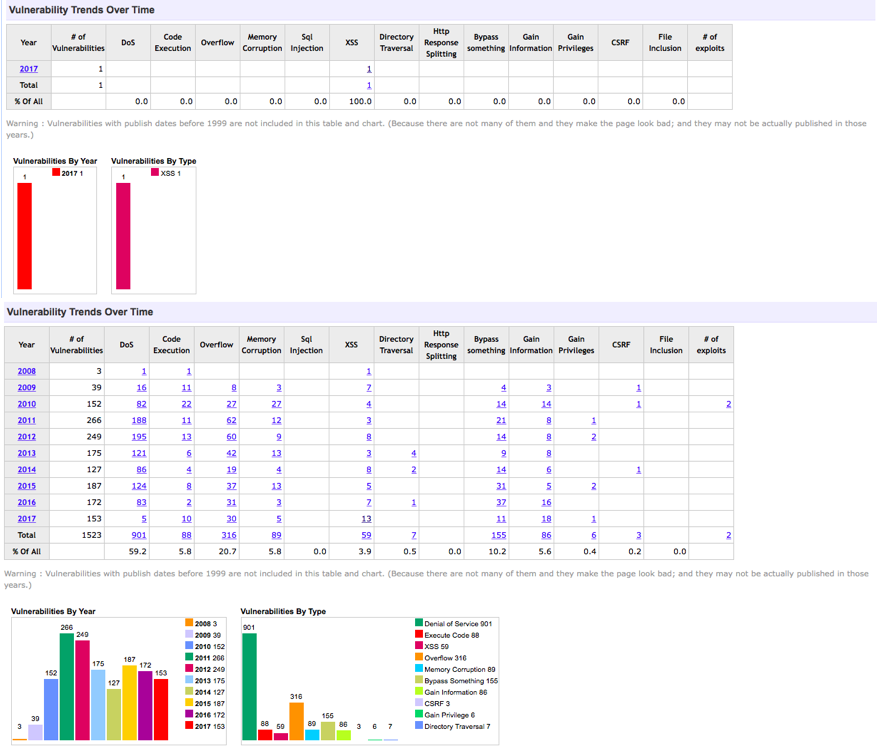
\includegraphics[width=0.47\textwidth]{images/BraveReportedVulnerabilities.png}
\caption{Brave Reported Vulnerabilities (top) compared to Google Chrome Reported Vulnerabilities (bottom) according to cvedetails.com}
\label{fig:BraveReportedVulnerabilities}
\end{figure}

\subsection{Environment specifications and software version}

Our project has been performed on a MacBook Air running macOS Sierra version 10.12.6, using the Brave version described in figure \ref{fig:BraveVersion}.

\begin{figure}[h]
\centering
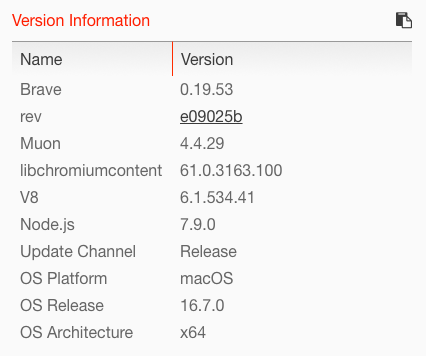
\includegraphics[width=0.4\textwidth]{images/BraveVersion.png}
\caption{Brave version used during our project}
\label{fig:BraveVersion}
\end{figure}


\subsection{Widening to other browsers}

Despite the fact that we first focused on Brave during this term project, we then decided to broaden our study to the other browsers listed below:

\begin{itemize}
\item \textbf{Whale} browser by Naver\footnote{http://whale.naver.com/en/}: version 1.0.37.16 (64-bit), released in October 23, 2017
\item \textbf{Firefox Quantum} by Mozilla\footnote{https://www.mozilla.org/en-US/firefox/}: Version 57.0 (64 bits), released in November 14, 2017
\item \textbf{Safari} by Apple: Version 10.1.2
\end{itemize}


\section{Our study}

\subsection{Scope of our study}

In the course of the last two months we investigated the causes of Universal Cross-Site Scripting in modern web browsers. As a consequence, we analyzed and studied the reported vulnerabilities that have been discovered on many browsers, in the course of the last years. 
As a wide panel of platforms are being used in our connected devices nowadays, we decided to eliminate from our study all vulnerabilities reported on mobile platforms such as iOS\footnote{https://en.wikipedia.org/wiki/IOS} or Android\footnote{https://en.wikipedia.org/wiki/Android\_(operating\_system)}. Such decision was due to the fact that security mechanisms are not exactly the same in mobile platforms than in laptop operating systems.

\medskip

In this section of the paper, we try to summarize the attacks we studied before. Then we seek to extract patterns that emerge from the attack scenario we studied. We conclude this passage by listing some of our attempts to bypass the security mechanisms of web browsers.

\subsection{Common Vulnerabilities and Exposures (CVE)}

In the previous part of the paper we explained how difficult securing a web browser was. Moreover, browser developers have to release new features in small amount of time to stay ahead of the competition. This makes testing an arduous task. Ensuring a full coverage of the software is almost impossible.

\medskip

In order to prevent attackers from exploiting potential flaws in web browsers and threaten users, companies decided to set up \emph{bug bounty programs}\footnote{https://en.wikipedia.org/wiki/Bug\_bounty\_program}. Such scheme consist giving \emph{"bug hunters"} a financial compensation and a high recognition for the bugs they report. That way, developers cooperate with part of the community and are able to discover and resolve bugs before the general public is aware of them. This helps preventing incidents of widespread abuse. \\
A majority, not to say all, of reported vulnerabilities have been classified in the Common Vulnerabilities and Exposures system which provides a reference-method for publicly known information-security vulnerabilities and exposures. \\

Most of the vulnerabilities we studied during this two-month research work are actually extracted from the CVE system. \\

In total we analyzed a set of nearly 80 vulnerabilities divided up as follow:

\begin{itemize}
\item 25 XSS vulnerabilities reported for Mozilla Firefox from 2012 to 2016, involving X version of the software
\item 30 XSS vulnerabilities reported for Google Chrome from 2009 to 2017
\item 7 XSS vulnerabilities reported for Internet Explorer and Edge from 2008 to 2016
\item 16 XSS vulnerabilities reported for Opera from 2008 to 2013
\item 1 XSS vulnerability reported for Brave in 2017
\end{itemize}

This set of vulnerabilities reported on 5 browsers in a time frame of 8 years, coupled with the study of disclosed vulnerabilities on web browser plugins, constituted the kernel upon which we based our study. The examination of these reported vulnerabilities helped us understand the different attack vectors used against web browsers. In addition, it helped us understanding the security mechanisms that have incrementally been implemented in web browsers in response of these successive attacks.

\medskip

Further to the the attack reports properly speaking, we took the time to read the discussions the development teams had on the vulnerability report, during the development of the patches. Not only following the developer's reasoning steps was very interesting, but also it made us realize the strict deadlines also referred to as \emph{"time-to-release"} the teams have to meet.


\subsection{Originality of attack scenarios}

The inspection of out vulnerability revealed an astounding wide range of attack scenarios, all more originals than the others. Such a variety of vulnerabilities is undoubtedly due to the complexity of web browsers and the large amount of possible exploitable flaws. From Cross Origin Drag and Drop \cite{CVE-2013-2849}, to SOP bypass using Reading mode \cite{edgeReadingModeUXSS}, UXSS from local MHTML\footnote{https://en.wikipedia.org/wiki/MHTML} files \cite{CVE-2014-1747}, or even exploit of vulnerabilities in plugins \cite{uxssPDF} \cite{uxssKeybase}, attackers are always more and more originals and manage to find breaches where to execute malicious scripts.

\medskip

Nevertheless, although we observed a huge variety of attacks, our analysis unveiled some sort of patterns common to multiple successful attacks against web browsers.

\subsection{Patterns of UXSS attacks}

An interesting part of our work has consisted in trying to find patterns in UXSS attacks. Despite the incredible diversity we observed in the CVE entries we examined, some vulnerabilities appeared to be exploited more regularly than others. \\
The following part of this section aims to list the popular attack vectors extracted from our study.

\medskip

\subsubsection*{\textbf{Extensions}}
Browser extensions are plug-ins that extend the features provided by a web browser. Extensions can be downloaded by users and integrated to their browsers to improve the user interface, the security or for blocking advertisements for instance. Such pieces of software have the right to access everything in the browser. This is the reason why, one should be really careful when it comes to use extensions, since any malicious could bypass the SOP and access sensitive data without efforts. To protect their users, many browsers have online stores that allow users to find extensions that have previously been verified. At this point 3 scenarios arise:
\begin{itemize}
\item The user installs a malicious extension from a malicious store: This exposes the user to dramatic attacks and data leaks. The extension developer is able to bypass the browser security mechanisms and access user's private data.
\item The user installs a malicious extension from a secure store: This case is less likely than the first case. Companies such as Google deployed mechanisms to detect malicious extensions and prevent them from being published on their store \cite{extensionsGoogle}. Nonetheless, in the case where a malicious extension manages to bypass all the checks, the consequences are the same as in the previous case. The user's private pieces of information are totally exposed to the attacker.
\item The user installs an official\footnote{By official we mean "non-malicious"} extension from a secure store. This case is the most interesting in our case. In such circumstances the user should be free from risks. However, this is not the case. If the attacker could not manage to find any vulnerability in the browser before, he can now try to find one in the extension. By using this "non-malicious" extension, the user gives the attacker another chance to attack him. Such weaknesses in extensions have been reported in Adobe Reader\cite{adobeExtensionUXSS}, or Keybase \cite{uxssKeybase} for instance. Finally, vulnerabilities can also be found in the part of the browser responsible for integrating the extensions \cite{CVE-2015-7187} \cite{CVE-2017-5020}.

\end{itemize}

\medskip

\subsubsection*{\textbf{Redirects}}

HTTP redirects are a special kind of HTTP response used for numerous goals such as temporary redirection while site maintenance is ongoing for instance. While this mechanism is, in general, implemented server side, web developers who do not have access over the server, can implement it in their HTML page (HTML redirections) or in their Javascript client (Javascript redirections). \\
Interestingly enough, carefully timed reloads and redirects can enable an attacker to bypass the SOP \cite{CVE-2015-0072}\footnote{In the PoC (https://blog.innerht.ml/ie-uxss/) of CVE-2015-0072, the author explains that JavaScript's single-threaded nature is actually used to freeze the browser with an alert box to actually manage to bypass the SOP}, \cite{CVE-2010-4045}, \cite{CVE-2009-3013}.

\medskip

\subsubsection*{\textbf{Diversity of URIs}}

In order to ensure good performances, and/or in order to support some features, web browsers come with numerous URIs. The \emph{data} URI scheme, for instance, is a uniform resource identifier scheme that provides a way to include data in-line in web pages as if they were external resources. Moreover, the \emph{feed} URI scheme is a URI scheme designed to facilitate subscription to web feeds; and the \emph{about} URI is an internal URI scheme implemented in various Web browsers used to reveal internal state and built-in functions. Such a variety of URIs has been widely used by attackers to carry out their attacks. Domainless \emph{about:blank} URIs have been used to bypass the SOP in \cite{domainlessAboutBlank}, while \emph{feed:} and \emph{data:} URIs have been used to execute malicious javascript code \cite{CVE-2012-1966} \cite{CVE-2012-1965} \cite{CVE-2011-2609} \cite{CVE-2012-6463} \cite{CVE-2010-2665}.

\medskip

\subsubsection*{\textbf{XSS Auditor}}

In order to avoid Cross-site Scripting attacks many web browsers implement a mechanism (XSS Auditor) using the \emph{X-XSS-Protection} HTTP header that is used to stop pages from loading when browsers detect reflected XSS attacks. In the case where the header is set to \emph{X-XSS-Protection: 1; mode=block}, once the auditor is triggered the response is blocked and a blank page is shown to the user.\footnote{https://www.virtuesecurity.com/blog/understanding-xss-auditor/}. This blocking mode in the XSS Auditor has also been an fairly "popular" attack vector used by attackers. Some scenarios exploited the fact that a page was blocked or not, to infer some secret information on a victim's page or to proceed to a document.referrer leakage \cite{CVE-2017-5045} \cite{CVE-2013-0909} \cite{CVE-2013-2848}

\medskip

\subsubsection*{\textbf{Cross Origin Drag and Drop/Copy and Paste}}

In HTML5, Drag and Drop has been included as part of the standard. Thus any element can be set as draggable, and custom events can be defined by the web developer to refine the behavior of his page during a drag and drop from the user. However, such a feature can be used in a malicious fashion. Attackers actually found scenarios where cross Drag and Drop were possible and thus lead to XSS conditions \cite{CVE-2016-5226} \cite{CVE-2013-2849} \cite{CVE-2012-0455}.

\medskip

\subsubsection*{\textbf{Malicious attributes values for DOM elements}}

The last method we observed, was frequently used to generate XSS conditions in web browsers was to confuse the browser with malicious names for DOM elements and/or malicious values for DOM elements' attributes. \\
In such case, the web browser's behavior could be changed and some security mechanisms could be altered. \\
Attacks that used this technique consisted in redefining global variable (variable clobbering\footnote{https://en.wikipedia.org/wiki/Clobbering}) \cite{frameBustingLocationClubbered}, escaping the browser XSS filters by writing some javascript payloads in the value of some DOM elements \cite{CVE-2013-2849}, or just naming an attribute with the name of a global variable \cite{CVE-2012-4209} \cite{CVE-2012-3994} \cite{CVE-2012-4194}

\bigskip

In addition of our observations during this research, \cite{uxssJSLeaks} provides an insighful analysis of UXSS vulnerabilities of the family of \emph{cross-origin JavaScript capability leaks}. In this paper, the authors carried out a study on WebKit\footnote{https://en.wikipedia.org/wiki/WebKit} and tried to detect and exploit when the browser leaked a JavaScript pointer from one security origin to another. They showed that the origins of such vulnerabilities came from the fact that the Document Object Model (DOM) and the JavaScript engine actually enforced the same-origin policy using two different security models: Access Control and Object-Capabilities. While Access Control, used by the DOM, prevents one Web site from accessing resources allocated to another Web site, the JavaScript engine enforces the same-origin policy using an object-capability discipline that prevents one Web site from obtaining JavaScript pointers to sensitive objects that belong to a foreign security origin. In their research they showed that is the browser leaked a JavaScript pointer from one security origin to another, this would lead to an exploitable vulnerability to bypass the SOP. 

\medskip

This study can actually be put into relation with the above section about \emph{Malicious attributes values for DOM elements}. Indeed, in this part we spoke about variable clobbering to prevent some security mechanisms to be triggered, such as frame busting scripts for instance. If, on the other hand, the attacker manages to overwrite some methods from a global Javascript object such as \emph{window} for instance, it would not be foolish to assume that, if invoked inside a victim iframe, this method would execute on behalf of the victim's origin. \\

Thus, it appears that, is some circumstances, and in some browsers, global variables could be seen as \emph{bridges} between origins, and used by malicious users to attack the web browser.


\subsection{Errors made by developers}

After studying the reported vulnerabilities found on today's most famous web browsers, and after extracting some common attack vectors - or patterns - used to attack these pieces of software, let's try to figure out some mistakes made from web browser developers.

\medskip

While some attacks exploit vulnerabilities that might not be easily predictable by the browser developers, some attacks could, however, be "easily" avoided. Some common mistakes made by browser developers could be:

\begin{itemize}
\item Lack of sanitization of user input: Could lead to script injection in URIs for instance.
\item Bad design of regular expression: Could allow a user to bypass some security checks. If the regular expression is case sensitive, a user could use upper and lower case letters to short-circuit any checks for instance \cite{CVE-2012-0455}
\item Divergence with specifications: Sometimes the specifications might add a lot of constraints on the developers. It might be tempting to "adapt" them. Nevertheless, such circumstances could create odd situations that could benefit an attacker \cite{CVE-2012-3985}
\item Confusion/Negligence: As browsers support a large panel of extensions, some situations appear when it is difficult to know the party responsible for the implementation of some security mechanisms. In case where an ambiguity happens, some security checks might be missing, allowing an malicious user to attack the software.
\item Inattention: By being focused on developing new features, web browser developers can mistakenly introduce regressions, and vulnerabilities that have already been patched. Thus an attacker might be able to carry out an old attack on the browser.
\end{itemize}

\medskip

\underline{\emph{Note:}} This list of potentials errors, is based on the messages exchanged on the bug report pages. 

\subsection{Our attempts}

Say that we tried to attack the browser but we stay at the surface (we didn't dove into implementation of the browser and didn't do an sort of analysis of the code to find flaws)

Say that we tried all our payloads against Brave, Whale, Google Chrome and Firefox Quantum -- Since all browsers are different, we wanted to try our payloads against them all. All browsers have their own set of features, so one might be unaffected by an attack while another can be vulnerable.

Based on the attacks we studied on a large range of browsers, we tried to carry out some attacks ourselves.
Speak about our different attempts here.
Further to the study of the patterns, we tried to do some UXSS attacks...
Say that none of our attempts were successful but that we provide them as a record of our work. They might also be extended/adapted to carry out successful attack.
Speak about what we tried, and why we tried it, and explain what we had in mind when we tried something (so that the reader can understand the attack more easily)
- In this part of the paper present some of our attempts. At least we can list what we tried, but we are not compelled to include all the payloads we came up with.

\subsection{Results}

We can say that all the payloads we crafted, and some precise results of our study are available on the github page of the project: https://github.com/KAIST-IS593-WEBSEC/UXSS-Vulnerabilities-Project
Conclude about the results of our attacks. Say that despite the fact that we couldn't find any vulnerabilities, the result should not be considered as null/bad --> we learnt a lot about some features used in web browsers/web apps, and we studied a large numbe rof attack scenario that we tried to reproduce. So it was a very exciting moment, sometimes fun (when we thought we were close to find a vulnerability), sometimes annoying (after a lot of failures) but the overall was very interesting for us to confront ourselves to the security mechanisms of today's web browsers. Trying to reproduce attacks, and trying to come up with our own paylaods undoubtedly helped us developing a deep understanding of today's web security mechanisms.

Conclude this section by saying that today's browsers are not trivially vulnerable (fortunately), however it is not because we didn't manage to find a vulnerability that no one is going to find one. 
Nevertheless, say that we are sure that we just broached the surface of all the possible attacks 

\subsection{Difficulties encountered}

--> Do a "Difficulties encountered" section and say that one difficulty we had was our lack of knowledge in web technologies and features exploitables in javascript/web browsers. This was on the one hand the most interesting part and the whole purpose of this project (discover and learn) but it also slowed us down a lot since we had to read a lot about what we could use to carry out an attack and know how to use it (ex: web workers, fetch API and all the things we discovered and tried to exploit)


\section{Conclusion}
Despite the fact that we didn't manage to find any vulnerability on the web browsers, some persons might be able to find some. It is important to remember that browsers act as a last rampart against malicious users/attackers. As many browsers are on the market today, the teams developing them are in a perpetual race against each other. The best browser is the most secure one with the most features to provide their users. However, as features are added to a browser, it is paramount to keep in mind the aspect of security.

[TO SAY FOR THE CONCLUSION]

- We learnt many things about web dev in this project: marquee html tag, X-XSS-PROTECTION, Many security mechanism, many attack scenarios, we also saw most of (not to say all) notions that have been presented this semester in this course (clickjacking, XSS, CSRF, UI timing attacks, browser extensions and so on) while we studied the previous attacks in the CVE record,

What we conclude from this study: UXSS will always occur/new vulns will always be found... --> Many =/= platforms, iOS, Android, Laptop (=/= OS) and so on + Browsers are extremely complicated software. The area for attackers to exploit potential vulnerabilities is really big (many things that can be exploited by attackers --> extensions, =/= internal components of the browser, third party component (cf: Blink/Webkit for instance), and so on...). The diversity of attacks is really really big. We though it would be easy to come up with patterns used to bypass the SoP, but it was not as simple as that. Some patterns can be detected, but this is not as obvious as we first thought.
We learnt a lot, we are not a team specilized/familiar with web development, but througout this study we were able to learn many things about UXSS attacks and about web development in general.
Moreover, while browsers provide users with a way to access resources plublished on the Web, they also ambed a very large number of features that make our web surfing way more agreable. In addition, they implement all sort of security mechanisms to prevent our personal/sensitive data from being accessed leaked out. Nevertheless, some of these mechanisms can be bypassed by attackers. Thus, these malicious users can tehn gain access to victim's sensitive data. That is the reason why web application developpers should not rely on browsers to secure their customer's data. Security on the web has to be handled and taken into consideration by everyone. Web app devs should define strict CSPs, use HTTPONLY cookies to prevent some javascript code from accessing them, do frame busting using the X-FRAME-OPTIONS header, use session IDs for a small amount of time, be careful with quick change of IP address when a user uses a webservice (at login and so on), use strong keys and encryption scheme for encrypted communications (see the paper "How DH fails in practice"), and keep on following the news in the web security areas while keeping their security infrastructure up to date.

-- We saw that a simple small error/lack of check of in a feature in a browser could lead to dramatic vulnerabilities that would threaten all users. A simple Drag and Drop and some malicious code could be added in an embedded/victim page and thus, some malicious code could be executed on his behalf.


To go further: Browsers developers might need to handle discrepancies in network traffic (see paper of SCA based on packet size), since personal data can also be leaked out further to network analysis of a passive attacker. So, despite all encrytpion and security mechanisms that are being implemented by browser developers, they might need to go a step further and hide our network trace to keep our data completelly safe. + (See paper about DH "How DH fails in practice" --> browser developers need to do a perpetual surveillance of what's going on in the security area and stop supporting deprecated Encryption schemeand so on.)

[TODO]
Say how many UXSS attacks we studied, and try to classify all these attacks into groups in order to get some insightful statistics and try to get the most used vulnerabilities to carry out UXSS attacks.



\section{IDEAS for the paper}
Note, while we were writing this paper, Mozilla released a brand new version of Firefox (Firefow Quantum). We didn't have time to test malicious payloads against this browser.
--> do some statistics about the UXSS attacks we saw/studied. For instance, 3\% of the UXSS we studied used vulnerabilities in plugins, 20\% managed to bypass the SOP by using embedded iFrames and blocked the browsers with server redirected, and so on --> try to find patterns of the attacks and the most used techniques to bypass the SOP -> do,such analysis for each browser and if we cannot manage to have decent stats -> speak about the different techniques we saw that were used to bypass the SOP.


--> Note: During the review of the different reported vulnerabilities, we read comments from reporter of the vulns but also the comments from the core team exchanging about how to fix the vulns --> During the reading of these messages, we really measured the pressure on the teams about releasing new versions of the software. It seems that time tables already contain day of release, and that the team has to cope with such delays and meet the deadlines. It seems there is a "time-to-release" pre-established.  

% if have a single appendix:
%\appendix[Proof of the Zonklar Equations]
% or
%\appendix  % for no appendix heading
% do not use \section anymore after \appendix, only \section*
% is possibly needed

% use appendices with more than one appendix
% then use \section to start each appendix
% you must declare a \section before using any
% \subsection or using \label (\appendices by itself
% starts a section numbered zero.)
%

% Can use something like this to put references on a page
% by themselves when using endfloat and the captionsoff option.

\begin{thebibliography}{1}

\bibitem{website}
https://www.brokenbrowser.com/uxss-edge-domainless-world/

\bibitem{paper1}
MJ Rees,
\textit{Evolving the Browser Towards a Standard User Interface Architecture}, 2001

\bibitem{DOM}
W3C,
\textit{Document Object Model (DOM)},
https://www.w3.org/DOM/

\bibitem{architectureWebBrowsers}
Alan Grosskurth, and Michael W. Godfrey,
\textit{A reference architecture for web browsers}, 2006

\bibitem{howBrowsersWork}
Tali Garsiel and Paul Irish,
\textit{How Browsers Work: Behind the scenes of modern web browsers}, 2011

\bibitem{browserSecurity}
Christoph Kerschbaumer,
\textit{Enforcing Content Security by Default within Web Browsers}, IEEE, 2016

\bibitem{SOP}
W3C,
\textit{Same Origin Policy (SOP)},
https://www.w3.org/Security/wiki/Same\_Origin\_Policy

\bibitem{CORS}
W3C,
\textit{Cross-Origin Resource Sharing (CORS)},
https://www.w3.org/Security/wiki/CORS

\bibitem{CSP}
W3C,
\textit{Content Security Policy (CSP)},
https://www.w3.org/TR/CSP/

\bibitem{SRI}
W3C,
\textit{Subresource Integrity},
https://www.w3.org/TR/SRI/

\bibitem{MixedContent}
W3C,
\textit{Mixed Content},
https://www.w3.org/TR/mixed-content/

\bibitem{browserSecurityWhitePaper}
Markus Vervier, Michele Orrù, Berend-Jan Wever, Eric Sesterhenn,
\textit{Browser Security White Paper},
X41 D-SEC GmbH, 2017
 
 
\bibitem{browserSecurityWhitePaper2}
Mario Heiderich,
\textit{Browser Security White Paper},
Cure53, 2017

\bibitem{isolationChrome}
The Chromium Projects,
\textit{Site Isolation},
https://www.chromium.org/developers/design-documents/site-isolation

\bibitem{uxssPDF}
Ofer Shezaf,
\textit{The Universal XSS PDF Vulnerability},
OWASP IL Chapter leader

\bibitem{uxssKeybase}
\textit{Universal Cross-Site Scripting in Keybase Chrome extension},
https://hackerone.com/reports/232432
 
\bibitem{webSecurityFoundation}
Devdatta Akhawe, Adam Barth, Peifung E. Lam, John Mitchell and Dawn Song,
\textit{Towards a Formal Foundation of Web Security}
 
\bibitem{javascriptSecurity}
Nataliia Bielova,
\textit{Survey on JavaScript security policies and their enforcement mechanisms in a web browser}
The Journal of Logic and Algebraic Programming, 2013

\bibitem{owaspXSS}
OWASP,
\textit{Cross-site Scripting (XSS)},
https://www.owasp.org/index.php/Cross-site\_Scripting\_(XSS),
2016

\bibitem{postMessagesXSS}
Son. et al. 
\textit{The Postman Always Rings Twice: Attacking and Defending postMessage in HTML5 Websites}, 
NDSS, 2013

\bibitem{uxssAcunetix}
Acunetix,
\textit{Universal Cross-site Scripting (UXSS): The Making of a Vulnerability},
https://www.acunetix.com/blog/articles/universal-cross-site-scripting-uxss/,
2014

\bibitem{braveWikipedia}
Wikipedia: Brave,
\textit{Brave (web browser)}
https://en.wikipedia.org/wiki/Brave\_(web\_browser),
2016

\bibitem{microsoftFuzzingOnv8}
Microsoft Offensive Security Research team,
\textit{Browser security beyond sandboxing},
https://blogs.technet.microsoft.com/mmpc/2017/10/18/browser-security-beyond-sandboxing/,
2017

\bibitem{xXssHeader}
Mozilla,
\textit{X-XSS-Protection},
https://developer.mozilla.org/fr/docs/Web/HTTP/Headers/X-XSS-Protection,
2017

\bibitem{CVE-2013-2849}
CVE-2013-2849,
\textit{Cross-Origin Copy \& Paste / Drag \& Drop allowing XSS},
https://bugs.chromium.org/p/chromium/issues/detail?id=171392,
2013

\bibitem{edgeReadingModeUXSS}
Manuel Caballero
\textit{SOP bypass courtesy of the reading mode (Edge)},
https://www.brokenbrowser.com/sop-bypass-abusing-read-protocol/,
2017

\bibitem{CVE-2014-1747}
CVE-2014-1747,
\textit{UXSS from a local MHTML file},
https://bugs.chromium.org/p/chromium/issues/detail?id=330663,
2014

\bibitem{uxssJSLeaks}
UC Berkeley,
\textit{Cross-Origin JavaScript Capability Leaks: Detection, Exploitation, and Defense}


\bibitem{extensionsGoogle}
Google,
\textit{Trends and Lessons from Three Years Fighting Malicious Extensions}

\bibitem{adobeExtensionUXSS}
CVE-2011-2107

\bibitem{CVE-2015-7187}
CVE-2015-7187

\bibitem{CVE-2017-5020}
CVE-2017-5020

\bibitem{CVE-2015-0072}
CVE-2015-0072

\bibitem{CVE-2010-4045}
CVE-2010-4045

\bibitem{CVE-2009-3013}
CVE-2009-3013

\bibitem{domainlessAboutBlank}
Manuel Caballero,
\textit{SOP bypass / UXSS – Adventures in a Domainless World (Edge)},
2017

\bibitem{CVE-2012-1966} 
CVE-2012-1966

\bibitem{CVE-2012-1965} 
CVE-2012-1965

\bibitem{CVE-2011-2609} 
CVE-2011-2609

\bibitem{CVE-2012-6463} 
CVE-2012-6463

\bibitem{CVE-2010-2665}
CVE-2010-2665

\bibitem{CVE-2017-5045}
CVE-2017-5045

\bibitem{CVE-2013-0909}
CVE-2013-0909

\bibitem{CVE-2013-2848}
CVE-2013-2848

\bibitem{CVE-2016-5226} 
CVE-2016-5226

\bibitem{CVE-2013-2849} 
CVE-2013-2849

\bibitem{CVE-2012-0455}
CVE-2012-0455

\bibitem{frameBustingLocationClubbered}
Gustav Rydstedt, Elie Bursztein, Dan Boneh and Collin Jackson,
\textit{Busting Frame Busting:
a Study of Clickjacking Vulnerabilities on Popular Sites},

\bibitem{CVE-2012-4209}
CVE-2012-4209

\bibitem{CVE-2012-3994}
CVE-2012-3994

\bibitem{CVE-2012-4194}
CVE-2012-4194

\bibitem{CVE-2012-0455}
CVE-2012-0455

\bibitem{CVE-2012-3985}
CVE-2012-3985

\end{thebibliography}

\ifCLASSOPTIONcaptionsoff
  \newpage
\fi



% trigger a \newpage just before the given reference
% number - used to balance the columns on the last page
% adjust value as needed - may need to be readjusted if
% the document is modified later
%\IEEEtriggeratref{8}
% The "triggered" command can be changed if desired:
%\IEEEtriggercmd{\enlargethispage{-5in}}

% references section

% can use a bibliography generated by BibTeX as a .bbl file
% BibTeX documentation can be easily obtained at:
% http://www.ctan.org/tex-archive/biblio/bibtex/contrib/doc/
% The IEEEtran BibTeX style support page is at:
% http://www.michaelshell.org/tex/ieeetran/bibtex/
%\bibliographystyle{IEEEtran}
% argument is your BibTeX string definitions and bibliography database(s)
%\bibliography{IEEEabrv,../bib/paper}
%
% <OR> manually copy in the resultant .bbl file
% set second argument of \begin to the number of references
% (used to reserve space for the reference number labels box)

% biography section
% 
% If you have an EPS/PDF photo (graphicx package needed) extra braces are
% needed around the contents of the optional argument to biography to prevent
% the LaTeX parser from getting confused when it sees the complicated
% \includegraphics command within an optional argument. (You could create
% your own custom macro containing the \includegraphics command to make things
% simpler here.)
%\begin{biography}[{\includegraphics[width=1in,height=1.25in,clip,keepaspectratio]{mshell}}]{Michael Shell}
% or if you just want to reserve a space for a photo:

% You can push biographies down or up by placing
% a \vfill before or after them. The appropriate
% use of \vfill depends on what kind of text is
% on the last page and whether or not the columns
% are being equalized.

%\vfill

% Can be used to pull up biographies so that the bottom of the last one
% is flush with the other column.
%\enlargethispage{-5in}



% that's all folks
\end{document}


